% Load the documentclass. thesis.sty was tested with book and scrbook
\documentclass{book}
% Load some useful packages for this document
\usepackage{graphicx}
\usepackage[final]{microtype}
\usepackage[utf8]{inputenx}
\usepackage{lmodern,mathpazo}
\linespread{1.05}
\usepackage[english]{babel}
\usepackage{colortbl,booktabs,blindtext}
\newcommand\thesis{\texttt{thesis.sty}}

\usepackage[
    backend=biber,
    sorting=none,
    url=false,
    doi=false
]{biblatex}
\addbibresource{uni22.bib}

% Farbdefinitionen
\definecolor{cadmiumgreen}{rgb}{0.0, 0.42, 0.24}
\definecolor{alizarin}{rgb}{0.82, 0.1, 0.26}
\definecolor{maroon}{rgb}{0.5, 0.0, 0.0}
%
\usepackage{enumitem}               % Ermöglicht verschiedene Aufzählungen (zb römisch)
%\usepackage[a4paper, left=3cm, right=3cm, top=3cm, bottom=3cm]{geometry}
\usepackage{textcomp}               % Winkelgrad, Minuten und Sekunden
\usepackage[onehalfspacing]{setspace}
\usepackage{graphicx}		        % Bilder
%\usepackage{floatflt}               % flt 
\usepackage{float}                  % Bindet Bilder genau da ein wo sie hin sollen (mit der Option H)
\usepackage[font={small}]{caption}  % Kleine Captions
\usepackage{amssymb}
\usepackage{amsmath}

\usepackage{listliketab}
\usepackage{tabto}
\usepackage{isotope} 
\usepackage{extarrows}
\usepackage{mathabx}
\usepackage{helvet}

%\usepackage{cite}
\usepackage{capt-of}
%\usepackage{unicode-math}
\usepackage{dsfont}
\usepackage{physics}
\usepackage[hidelinks]{hyperref}
\usepackage[nameinlink, english]{cleveref} 
\crefname{ineq}{ineq.}{inequalities}
\creflabelformat{ineq}{#2{\upshape(#1)}#3}
\crefname{def}{def.}{def.}
\creflabelformat{def}{#2{\upshape(#1)}#3} 
%\crefname{equation}{Gleichung}{Gleichungen} % bringt nichts
%\crefname{figure}{Abbildung}{Abbildungen}

%%%%%%%%%% Plotten und Zeichnungen,...
%\usepackage{gnuplottex}
%\usepackage[miktex]{gnuplottex}
\usepackage{pgfplots}			% Nutzung wenn matlab2tikz oder maplotlib2tikz
\pgfplotsset{compat=newest}	% bzw. tikzplot verwendet wird|| compat=1.16 tut auf
							% jeden Fall.
%\usepackage{pgf} % Nicht zwingend nötig...
\usepackage{tikz}
\usepackage{pgfplots}
%\usepackage{pst-all} %TODO %TODO %TODO %TODO %TODO %TODO %TODO %TODO
%\usepackage{pstricks} % Die hier müssen auskomentiert sein.
%%%% Die machen mit tikz Ärger. Vor allem mit der pattern library.
%\usepackage{pst-plot} %TODO %TODO %TODO %TODO %TODO %TODO %TODO %TODO
\usetikzlibrary{angles,quotes,calc,automata,positioning,patterns,external, hobby, shapes.misc}
\usepgfplotslibrary{fillbetween} %Ausfüllen von Flächen zwischen Funktionen in pgfplots plots -REH
\tikzset{cross/.style={cross out, draw=black, minimum size=2*(#1-\pgflinewidth), inner sep=0pt, outer sep=0pt}, cross/.default={2.5pt}} %Defines crosses for Tikz-plots -REH
\usepackage{ifthen}
\usepackage{tikz-3dplot}
\usetikzlibrary{fadings, intersections, decorations.pathreplacing}
\usetikzlibrary{matrix, math, snakes}
\usepgfplotslibrary{fillbetween}
\usepackage{tikzorbital}
\usepackage{pgflibrarysnakes}

%%%%% Tikz-Grafiken externalisieren
\usetikzlibrary{external}
\tikzexternalize[prefix=tikz/]
%\tikzexternalize[prefix=tikz/,optimize command away=\includepdf]
% ... Wegoptimieren kann nützlich sein, muss aber nicht.
% Hier würde es die Grafiken verkleinern, was ungewollt wäre.
\makeatletter							% Definition eines Kommandos, das so nicht
\newcommand{\useexternalfile}[1]{%		% zwingend benötigt wird
    \tikzsetnextfilename{#1-output}%
    \input{\tikzexternal@filenameprefix#1.tikz}}
\makeatother
%%%%%%%%%%
% TikZ sucht im Ordner 'TikZ' nach den .tikz-Dateien und lädt sie bzw.
% die aus ihnen generierten .pdf-Dateien. Falls eine Änderung in der .tikz-Datei
% detektiert wird, wird diese im Dokument neu 'kompiliert'. Falls nicht, wird
% die oben erwähnte .pdf-Datei verwendet, die nach dem 'Kompilieren' im
% TikZ-Ordner gespeichert wird.
%
%TODO WICHTIG ist, dass die entsprechende Datei ohne Endung eingebunden wird
%TODO		  und sich im TikZ-Ordner befindet.
%
% Der Befehl
% 			\tikzexternalize[prefix=tikz/]
% erzeugt im Ornder 'tikz' .pdf-Dateien von tikz-Grafiken. Einmal erstellt, werden
% diese nur nach detektierten Änderungen neu erstellt.
% Wird in prefix=tikz/ tikz geändert, so kommen die Ausgabedateien in einen
% generierten Ordner mit dem geänderten Namen. Existiert bereits ein Ordner mit
% diesem Namen, so wird der Inhalt ergänzt.
% Die Befehle
% 			\tikzexternaldisable und
% 			\tikzexternalenable
% heben die Wirkung von \tikzexternalize[] auf bzw. lassen den Befehl wieder wirken.
% Der Befehl
%			\tikzsetnextfilename{}
% ändert den Standarddateinamen der von tikzexternalize erzeugten .pdf-Datei
% zum Klammerinhalt.
\tikzexternaldisable



\numberwithin{equation}{section} % Nummeriert die Gleichungen mit jeder section neu

% Load thesis.sty
\usepackage[consistency,dottedtoc,styledtoc]{thesis}


\chapterboxheight=15ex
\chapterboxwidth=10em

\usetikzlibrary{patterns,intersections,snakes}

\title{Thermodynamic cost of quantum information} %TODO
\author{Etienne Maurice Springer}% don't use \and
\university{\textls{University of Stuttgart}}
\city{Stuttgart}
\date{29 July 2022}
\thesisname{Bachelor's Thesis}
\institute{Institute for Theoretical Physics I}
\supervisor[Supervised by]{Finn Schmolke}
\supervisor[Examiner]{Prof. Dr. Eric Lutz}

\begin{document}

% This is a sample titlepage design
\makethesistitle

\tableofcontents
\chapter{Introduction}
\textbf{TODO: THIS SECTION}
\begin{itemize}
    \item classical information theory and thermodynamics 
    \item something something maxwell demon, information is physical \cite{BA_maxwelldemon}
    \item landauer's principle \cite{HS_BA_landauer1961irreversibility}
    \item quantum information \& quantum thermodynamics
    \item bound on information flow pendry \cite{BA_Pendry_1983}
    \item nowadays correlations become physically realizable \cite{BA_kaonan_correlations}
    \item bound on information flow with these correlations?????
\end{itemize}
Although the theory of thermodynamics is more than 150 years old 
(for reference, Maxwell's \emph{Theory of heat} was released in 1872 \cite{BA_maxwelldemon}),
it seems to contradict itself by creating perpetual motion machines in the minds of physicists.
Most recently, with the advent of fluctuation theorems such as Crooks FT \cite{BA_CROOKS-fluctuation}
or Jarzynski's Relation \cite{HS_Jarzynski_1997} marking the dawn of stochastic thermodynamics, \cite{HS_BA_Seifert_2012}
thermodynamics is one of the hottest fields in theoretical physics today.\\

One milestone result in its history is the connection between energy dissipation and irreversibility in
computation. A spectre was haunting late 19th and early 20th century physicists, a spectre of James Clerk Maxwell.
A demon, to be precise.

This thesis is about limits on the flow of information

\chapter{Theoretical Basics}
This chapter gives the reader a brief overview of 
the mathematical formalism behind quantum mechanics and touch on the postulates
of quantum mechanics such as the state vector, the description and measurements of physical quantities 
and the Schrödinger equation.
We will then outline the notion of the thermodynamic quantities heat, work and internal energy
in quantum systems.
Finally we get into some specific measures of quantum information theory.
A reader already familiar with the basics of quantum thermodynamics is invited to skip these passages.

\emph{For the sake of simplicity, the reduced Planck constant $\hbar$ and Boltzmann's constant $k$ are set equal to 1.}

\section{The Basics of Quantum Mechanics}

\subsection{State Vector Formalism}\label{sec:statevector}
 %TODO
%The time evolution of this system is given by the phase space trajectory, $\vb*{\xi}(q_i,p_i;t)$.
%The phase space can be thought of as $\mathbb{R}^n$ with $n$ degrees of freedom in the system.\\
In classical Hamiltonian mechanics the state of a system (at some time $t$) is represented by a point $\xi$ in phase space,
which, for a system with $n$ degrees of freedom, resides in $\mathbb{R}^{2n}$\cite{BA_Nolting2014}.\\
According to the first postulate of quantum mechanics, the state of a system (at time $t$) is defined by a unit
vector in Hilbert space $\mathcal{H}$, called \emph{state vector} \cite{BA_cohen_tannoudji}.
This gives rise to an intriguing fundamental difference to the classical world,
since any arbitrary vector (in $\mathcal{H}$) can be represented as a linear combination of basis vectors.
This is called the superposition principle \cite{BA_Poschel2015,BA_messiah2014quantum}.
%Formulating this into an equation, it is customary to use the Dirac- (or Bra-Ket-) notation.
%The vector representing state $\psi$ becomes $\ket{\psi}$\footnote{read: Ket $\psi$. Also called \emph{Ket-vector}}.
Let us consider the fundamental example of a two-state system, with a ground state '0' and an excited state '1'.
The most general state of the system is described by a superposition of the two states,  
\begin{align}\label{eq:superpos}
    \ket{\psi} = c_1 \ket{0} + c_2 \ket{1}.
\end{align}
In \cref{eq:superpos}, quantum states are represented using the so-called Bra-Ket-notation. 
The state vector of a quantum system in $\mathcal{H}$ is denoted by $\ket{\psi}$\footnote{read: Ket $\psi$. Also called \emph{Ket-vector}},
with the corresponding vector $\bra{\psi}$\footnote{read: Bra $\psi$. Also called \emph{Bra-Vector}} in dual space.
The inner product on $\mathcal{H}$ is then defined as
$\braket{\varphi}{\psi}$.
\par
Since states are elements of a complex vector space, they are physical observable quantities. Therefore, the formalism
has to be complemented with a mathematical formalism of observables in order to get a complete and meaningful description of quantum systems.
In general, physical quantities can be measured (observed) and the outcome of such a measurement should therefore be
a real\footnote{as opposed to complex} number.
For this we employ the second postulate of quantum mechanics. It states that measureable physical quantities
(observables) are hermitian operators acting in $\mathcal{H}$. %\cite{BA_cohen_tannoudji}
The hermitian property implies that the operator only has real eigenvalues, is diagonalizable,
and that its eigenvectors are orthogonal \cite{BA_messiah2014quantum}.\\
%We measure by applying an operator of an observable $\hat{A}$ to the state vector $\ket{\psi(t)}$ is called measuring.
Let us convince ourselves of the advantages that come with this hermitian property.
Suppose we want to measure some observable $A$.
The outcome of such a measurement is an eigenvalue $a_k$ of the operator $\hat{A}$. The probability to observe the specific outcome $a_k$ is
\begin{align}\label{eq:prob-meas}
    p(a_k) = \braket{\psi}{a_k}\braket{a_k}{\psi} = \abs{\braket{a_k}{\psi}}^2,
\end{align}
where $\bra{a_k}$ are the eigen-bras of $\hat{A}$ with eigenvalue $a_k$.\\
Due to the inherent probabilistic description of quantum mechanics (cf. \cref{eq:prob-meas}), we can only make meaningful statements about averages.
Weighing every eigenvalue $a_k$ with its respective probability to be measured given by \cref{eq:prob-meas}, the average of an observable becomes \cite{BA_HS_nielsenchuang}
\begin{align}
    \expval{\hat{A}} = \sum\limits_k a_k p(a_k) = \sum\limits_k a_k \braket{\psi}{a_k}\braket{a_k}{\psi}
    = \bra{\psi} \left(\sum\limits_k a_k \dyad{a_k}\right) \ket{\psi} = \ev{\hat{A}}{\psi}.
\end{align}\\
Let us consider a concrete example of an operator.
Arguably the most essential operator in quantum mechanics is the Hamilton operator $\hat{H}$, often simply abbreviated as Hamiltonian.
It describes the total energy of a system, and is the generator of time translation, i.e. time evolution. A state vector evolves
according to the \emph{Schrödinger equation}, defined as \cite{BA_messiah2014quantum}
\begin{align}\label{eq:schro-eq}
    i\partial_t \ket{\psi(t)} = \hat{H} \ket{\psi(t)}.
\end{align}
Solving \cref{eq:schro-eq} gives us
\begin{align}\label{eq:schro-sol}
    \ket{\psi(t)} = e^{-i\hat{H}t}\ket{\psi(0)} \equiv U(t)\ket{\psi(0)}
\end{align}
with $U(t)$ defined as the unitary time evolution operator. Unitary operators fulfil the relation $UU^\dagger=\mathds{1}$, i.e.
its inverse is given by its adjoint. Using the fact that the Hamiltonian is a hermitian operator, unitarity follows from 
\begin{align}\label{eq:unitary-property}
    U(t)U^\dagger(t) = e^{-i\hat{H}t}e^{i\hat{H}^\dagger t} = e^{-i\hat{H}t}e^{i\hat{H}t} = \mathds{1}.
\end{align}
The determinant of such an operator is $1$, meaning that
the state vector the operator acts upon keeps unit length during its time evolution.
\par
In \cref{eq:schro-sol} and \cref{eq:unitary-property} we used the exponential of an operator. Since the
product of operators and
the series expansion of the exponential function are well defined, the exponential of an operator is defined through series expansion.
For instance, the series expansion of $U(t)$ becomes
\begin{align}\label{eq:matrix-exp}
    U(t) = \sum\limits_{n=0}^\infty \frac{(-i\hat{H}t)^n}{n!}.
\end{align}
\subsection{Density Matrix Formalism}\label{sec:densitymatrix}
Sometimes when describing quantum states, we prefer not to use state vectors, but instead use density matrices.
Density matrices (or density operators) come with some useful benefits over state vectors.
They let us describe correlations, thermal states (cf. \cref{sec:thermal-states}), and entropic quantities (cf. \cref{sec:entropy-rel-quant}), which
are the building blocks of quantum thermodynamics as well as quantum information theory.
Let us now extend the postulates of the previous section to density matrices.\\
%Consider a system with quantum states $\ket{\psi_k}$ and probabilities $p_k$ to be in the respective state $\ket{\psi_k}$.
%The density matrix of such a system is then defined as
Consider a system with a complete basis set of state vectors $\{\ket{\varphi_k}\}$. 
Now imagine that we fail to prepare our system in one of the specific states $\ket{\varphi_k}$ because of the temperature of the environment.
Then, we rather obtain a probabilistic mixture of the pure states $\dyad{\varphi_k}$ where each of the pure states has a classical probability $p_k$ to be observed.
In this case we introduce
\begin{align}\label[def]{def:densitymatrix}
    \rho \equiv \sum\limits_kp_k\dyad{\varphi_k}
\end{align}
as the \emph{density matrix} (sometimes also \emph{statistical operator}) of such a system \cite{BA_breuer2002theory}. \\
Following from \cref{def:densitymatrix}, we can ascribe certain properties to density matrices. These include
\begin{align}
    \Trace[\rho] &= 1,\label{eq:rho-trace-one}\\
    \Trace[\rho^2] &\leq 1,\label{eq:rho-squared-leq-one}\\
    \rho^\dagger &= \rho.\label{eq:rho-hermitian}
\end{align}
States that fulfil the equality in \cref{eq:rho-squared-leq-one} are called \emph{pure states}. Otherwise states are called \emph{mixed states}.\\
A measurement 
In our formalism, this is defined as
\begin{align}\label[def]{def:expval-a-rho}
    \expval{\hat{A}} \equiv \Trace[\rho \hat{A}]
\end{align}
for an observable $\hat{A}$.
Using the Hamilton operator as an example, we can define the mean energy of a system, namely
\begin{align}
    \expval{\hat{H}} = \Trace[\rho \hat{H}]\equiv E.
\end{align}
We already know that the Hamiltonian of a system generates the time evolution of a state according to the Schrödinger equation,
\cref{eq:schro-eq}.
We now want to know the time evolution of a system, which we describe initially with the density matrix
\begin{align}\label{eq:rho-at-time-zero}
    \rho(0) = \sum\limits_k \omega_k \dyad{\psi_k(0)},
\end{align}
where $\ket{\psi_k(0)}$ is an arbitrary state vector at time $t=0$.
At this point it is important to pay attention to fact that the $p_k$ of \cref{def:densitymatrix} and $\omega_k$ of \cref{eq:rho-at-time-zero}
describe different probabilities. While $p_i$ describes the classical probability of the system to be in the \emph{basis} state
$\ket{\varphi_i}$, the $\omega_i$ describes the probability of the system to be in an arbitrary state $\ket{\psi_i}$ if the system is
in a mixture of states $\ket{\psi_k}$ \cite{BA_messiah2014quantum, BA_breuer2002theory}.
Applying the unitary operator $U(t)$ introducted in \cref{eq:schro-sol} to \cref{eq:rho-at-time-zero} we get
\begin{align}\label{eq:rho-of-t}
    \rho(t) = \sum\limits_k \omega_k \left[U(t)\dyad{\psi_k(0)}U^\dagger(t)\right] = U(t) \rho(0) U^\dagger(t).
\end{align}
Taking the derivative with respect to time of \cref{eq:rho-of-t} we get
\begin{align}\label{eq:vn-eq}
    i\partial_t \rho(t) = \hat{H}\rho(t) - \rho(t) \hat{H} \equiv \comm{\hat{H}}{\rho(t)}.
\end{align}
\Cref{eq:vn-eq} is known as the \emph{von Neumann equation} and is the quantum mechanical analogue to the Liouville equation
from classical mechanics.

\subsection{Composite Systems}
\textcolor{red}{\textbf{TODO: THIS SECTION, AGAIN}}\\
%A composite system is a system which consists of multiple subsystems.
Many problems of quantum mechanics not only involve a single system, but multiple systems interacting with each other.
In this case it is more convenient to consider the interacting systems as part of one large composite system
and describe the physics from the top level of the composite density matrix and from there compute the quantities
of the individual subsystems.
We now want to --- phenomenologically --- construct the density matrix of such a composite system.\\
Let us first consider the simplest example: two qubits, denoted $A$ and $B$, with 
respective ground and excited states $\ket{0}_{A(B)}$ and $\ket{1}_{A(B)}$. Each individual system $i$
exists within a separate Hilbert space $\mathcal{H}^i$ with density matrix
\begin{align}
    \rho^i = p_0^i \dyad{0}_i + p_1^i \dyad{1}_i.
\end{align}
This way, the probability to, for example, find system $A$ in state $\ket{0}_A$ is $p_0^A$.\\
Suppose we let these systems interact with each other.
Instead of two (independent) systems with two states, we consider one composite system $\rho^{AB}$ with four states.
Consequently, the Hilbert space of this system becomes a combination of the two separate spaces $\mathcal{H}^{AB}$.
Since we are now dealing four states, the pure states of the composite system are different and will
therefore have different classical probabilities as well.
For instance, the composite system gives answers to the question how likely it is to find A and B simultaneously
in specific states, e.g. the probability to find A in the excited and B in the ground state $\ket{01}_{AB}$.
From a statistical point of view, the answer to this question
should simply be the product of the two separate probabilities $p_0^A$ and $p_1^B$ \cite{HS_BA_SeifertSkript}\footnote{This holds only for independent
probabilities, but because we ask about the systems initially, this holds true.}. %TODO, cite some textbook
Taking these probabilities into account and labeling the states appropriately, we can construct the density matrix of the composite system.
We get
\begin{align}\label{eq:compsys-rhoAB-initial}
    \rho^{AB} = p_0^Ap_0^B \dyad{00}_{AB} + p_0^Ap_1^B \dyad{01}_{AB} + p_1^Ap_0^B \dyad{10}_{AB} + p_1^Ap_1^B \dyad{11}_{AB}
\end{align}
for our initial density matrix. The kets $\ket{\cdot}_{AB}$ function as basis vectors for the combined Hilbert space $\mathcal{H}^{AB}$.
The probabilities of our density matrix evolve in time governed by \cref{eq:vn-eq}, where the interaction may be taken into account
by some Hamiltonian $\hat{H}_\text{int}$.\\

% The proper way to compute its density matrix
%is by performing the Kronecker product on the density matrices of the elements of this system, i.e.
%\begin{align}
%    \rho_\text{system} = \bigotimes\limits_{i=1}^N \rho_i.
%\end{align}


\subsection{Entanglement}
\textcolor{red}{\textbf{TODO: COHERENCE/CORRELATIONS}}
what


\subsection{Pauli Matrices}
\textcolor{red}{\textbf{TODO: THIS SECTION}}
Pauli matrices:

\begin{align}
    \sigma^x = \pmqty{\mqty{\pmat{1}}} \ \ \sigma^y = \pmqty{\mqty{\pmat{2}}} \ \ \sigma^z = \pmqty{\mqty{\pmat{3}}}
\end{align}

\subsection{Spin Chains}
\textcolor{red}{\textbf{TODO: SPIN CHAINS}}
\textcolor{red}{czycholl theo festk physik, kapitel 6 abschnitt 5ff}

\section{Basic notions of quantum thermodynamics}
\subsection{Thermal states}\label{sec:thermal-states}
The quantum counterpart of the Gibbs-Boltzmann distribution of the canonical ensemble is the Gibbs statistical ensemble. We will refer to it
as thermal state. It gives the equlibrium state of a quantum system with Hamiltonian $\hat{H}$ at inverse temperature $\beta$
and is defined as \cite{BA_Alicki2018}
\begin{align}\label[def]{def:therm-state}
    \rho_{th} \equiv \frac{1}{\mathcal{Z}}e^{-\beta\hat{H}} \qq{with the partition function} \mathcal{Z} = \Tr[e^{-\beta\hat{H}}].
\end{align}
In the eigenbasis $\{\ket{n}\}$ of the Hamiltonian we can perform a spectral decomposition and write
\begin{align}\label{eq:rho-therm-eigbasis}
    \rho_{th} = \sum\limits_n e^{-\beta E_n} \dyad{n}
\end{align}
\textcolor{red}{\textbf{TODO: FIND CITATION FOR THIS OR PUT DERIVATION IN APPENDIX}}
\subsection{The first law of thermodynamics}
\textcolor{red}{\textbf{TODO: THIS SECTION}}
First law:
\begin{align}
    \dd E = {W} + {Q}
\end{align}
Time dependent quantities:\cite{BA_Alicki_1979}
\begin{align}
    E(t) &\equiv \Tr[\rho(t)(H_0+H_t)]\label[def]{def:mean-energy-qtd}\\
    Q(t) &\equiv \int\limits_0^t\dd\tau\Tr[\dv{\rho(\tau)}{\tau} \left(H_0 + H_\tau\right)]\label[def]{def:heat-qtd}\\
    W(t) &\equiv \int\limits_0^t\dd\tau\Tr[\rho(\tau)\dv{H_\tau}{\tau}]\label[def]{def:work-qtd}
\end{align}
In the case of $H_t = 0$ the work vanishes and the mean energy becomes equal to $Q$
\newpage
\section{Entropy and quantum information}
Entropy is the essential concept of classical information theory.
It is a measure of information itself and paves the way for other measures of information-
and probability theory.
It is therefore only natural to imagine quantum equivalents of these well established classical quantities.
The following sections will introduce the most important quantum equivalents.
We will furthermore show the derivation of a fundamental inequality found by Pendry \cite{BA_Pendry_1983}, where the energy
current provides an upper bound to the flow of information. This relation is the main focus of this thesis.
\subsection{Entropy and other related quantities}\label{sec:entropy-rel-quant}
Unless otherwise stated, this section is losely based on the introductions of the respective quantities in
\citetitle{BA_HS_nielsenchuang} by \Citeauthor{BA_HS_nielsenchuang},
but uses logarithms base $e$ instead of base 2
to agree with the units used in the other references cited throughout this work,
especially the works of \citeauthor{BA_Pendry_1983} \cite*{BA_Pendry_1983} and \citeauthor{BA_kaonan_correlations} \cite*{BA_kaonan_correlations}.\\
We first briefly revisit the classical definitions of informational quantities.
Consider the discrete probability distributions $p_x$ and $q_x$ on the same set of elements $\{x\}$.
\paragraph{(Self-)Information}
\begin{align}
    I(p_x) \equiv -\ln(p_x)
\end{align}
The \emph{self-information} of a random variable $x$ defines the information one obtains after $x$ happens or is measured.
It quantifies how uncertain we are about $x$ happening \cite{BA_shannon}.
This definition can also be interpreted as \emph{surprisal}, i.e. how surprised we were after $x$ happened.
As an example, consider the roll of an unfair die. For this die the individual probabilities are $1/4$ for odd numbers and $1/12$ for even numbers.
The uncertainty of rolling a $6$ is $I(p_6) = -\ln(1/12) = \ln(12) = 2\ln(2) + \ln(3)$.
\paragraph{Shannon entropy}
\begin{align}\label[def]{def:shannon}
    S[p_x] \equiv - \sum\limits_x p_x \ln(p_x)
\end{align}
The Shannon entropy is defined as a quantity that measures how uncertain we are about a
measurement given a probability distribution \cite{BA_shannon}.
The crucial difference between entropy and information is that information defines the uncertainty
of measuring one particular $x$, while entropy is the average uncertainty before measuring.
Another way to interpret entropy is as the average minimum number of yes/no questions needed to know the outcome of the measurement,
multiplied by $\ln2$ \cite{HS_BA_SeifertSkript}.
Consider the example of two friends, Alice and Bob, playing with the die from before. Alice rolls the die and Bob, knowing the probabilities,
guesses the outcome.
The Shannon entropy, or average uncertainty, becomes
\begin{align}\label{eq:shannon-example}
    S[p_x] = - 3\cdot\frac{1}{4}\ln(\frac{1}{4}) - 3 \cdot\frac{1}{12}\ln(\frac{1}{12}) = 2\ln(2) + \frac{1}{4}\ln(3).
\end{align}

%In the literature you may find $H(x)$ used for entropy with natural log.
\paragraph{Kullback-Leibler Divergence} 
\begin{align}\label[def]{def:kld-classical}
    \mathcal{D}[p_x\mid\mid q_x] \equiv \sum\limits_x p_x\ln(\frac{p_x}{q_x}) = -S[p_x] - \sum\limits_x p_x\ln(q_x)
\end{align}
The \emph{Kullback-Leibler Divergence}, sometimes refered to as \emph{relative entropy}, is a measure for how different two distributions are.
In the information theoretical context it can be seen as the additional average uncertainty for an event with probability distribution $p_x$
if one falsely assumes $q_x$ to be the probability distribution for such event \cite{HS_BA_SeifertSkript, BA_kl-divergence}.
Suppose Alice and Bob play the game of the previous example. Unaware of the fact that it is rigged, Bob assumes an even distribution of probabilities.
The average uncertainty about a measurement now increases, 
\subsubsection{Von Neumann entropy}
Shannon entropy defines the average uncertainty of a probability distribution.
In order to obtain a measure for quantum entropy, we replace the classical probability distributions by the statistical operator
--- the density matrix --- $\rho$.
The average of a quantum observable is defined in \cref{def:expval-a-rho}.
Na{\"i}vely, we could then just plug the negative log of a density matrix $-\ln(\rho)$ as observable $\hat{A}$
into \cref{def:expval-a-rho} to get the entropy.
Formally, we get
\begin{align}\label{eq:naive-q-ent}
    \expval{-\ln(\rho)} = -\Trace[\rho\ln(\rho)].
\end{align}
It turns out that the right hand side of \cref{eq:naive-q-ent} is the entropy defined by von Neumann.
We may therefore define the \emph{von Neumann entropy} as
\begin{align}\label[def]{def:vn-ent}
    S(\rho) \equiv -\Trace[\rho\ln(\rho)].
\end{align}
Notice that in \cref{def:vn-ent} the argument of the logarithm is now a matrix.
In general, functions of matrices are calculated through series expansion.
If $\rho$ has eigenvalues $\lambda_k$, \cref{def:vn-ent} can be written as
\begin{align}\label{eq:vn-ent-eigval}
    S(\rho) = - \sum\limits_k \lambda_k \ln(\lambda_k).
\end{align}
It is easy to see from \cref{eq:vn-ent-eigval} that if our system is in a pure state, i.e. $\lambda_j = 1$, $\lambda_{i\neq j} = 0$,
the entropy of this state is 0. A way to interpret this result is that the uncertainty about our system is 0. We know our system
to be in the pure state.
Additionally, since $\Tr[\rho]=1$ and $0 \leq \lambda_k \leq 1$, the von Neumann entropy is non-negative
and 0 iff. $\rho$ is a pure state.\\
For a thermal state $\rho = rho_{th}$ on the other hand, as discussed in \cref{sec:thermal-states}, we get
\begin{align}\label{eq:therm-ent}
    S(\rho_{th}) = - \expval{\ln(\rho_{th})}
    = - \expval{\ln(\frac{e^{-\beta\hat{H}}}{\mathcal{Z}})}
    = \beta\expval{\hat{H}} + \ln(\mathcal{Z}) = \beta E + \ln(\mathcal{Z}),
\end{align}
with the system's mean energy $E = \Trace[\rho \hat{H}]$.
We find that within our framework, the entropy of the thermal state $\rho_{th}$ is identical to the entropy of a
canonical distribution $S = \beta(U-F)$ with mean energy $U$ and $F=\beta^{-1}\ln(Z)$ \cite{HS_BA_SeifertSkript}.
This is the expected behaviour, because we defined our state as the quantum analogue of the canonical distribution.
Then we calculated its entropy, which was derived a priori using the classical definition of entropy.
In a sense, this tells us that our notions of entropy and thermal states are consistent with already established frameworks of statistical mechanics.
\subsubsection{Kullback-Leibler Divergence}
The Kullback-Leibler Divergence, or \emph{relative entropy}, is a measure for how different two
probability distributions are. Its value is 0 if and only if the two distributions are identical \cite{HS_BA_SeifertSkript}.
The Kullback-Leibler divergence (KLD) of two density matrices $\rho$ and $\sigma$ is defined as
\begin{align}\label[def]{vn-}
    S(\rho\mid\mid\sigma) \equiv \Trace[\rho\ln(\rho)] - \Trace[\rho\ln(\sigma)] = - S(\rho) - \Trace[\rho\ln(\sigma)],
\end{align}
with the von Neumann entropy $S(\rho)$.
This definition agrees with what we expect from replacing $p_x$ with $\rho$ and $q_x$ with $\sigma$ in
\cref{def:kld-classical}.
%Analogous to the classical relative entropy, the quantum relative entropy
%describes how different two quantum states are.
%It is 0 iff. the two density matrices $\rho$ and $\sigma$ correspond to the same state.
In a information theoretical context the quantum relative entropy is the ammount of additional average uncertainty we get
given that we falsely assume our system to be described by $\sigma$ instead of $\rho$.
If two states are identical there is no additional uncertainty and the relative entropy vanishes.
\subsubsection{Fidelity}
\textcolor{red}{\textbf{TODO: THIS SECTION\\WHICH DEFINITION DOES QUTIP USE?}}
\begin{align}
    F(\rho,\sigma) = \Tr[\sqrt{\sqrt{\rho}\sigma\sqrt{\rho}}]
\end{align}
\subsection{Limits to the flow of quantum information}
%\textcolor{red}{\textbf{QUESTION: DO I USE $\vb{\hbar}$ FOR THE DERIVATION?}}\\
The central relation discussed in this work is the inequality derived by J. B. Pendry in 1983. In this section we will
sketch his original derivation. Consequently, this section will follow ref. \cite{BA_Pendry_1983}.\\
Suppose we are to detect $N$ bits of information during some time $t$. The energy-time uncertainty relation tells us that \cite{BA_Mandelstam1991}
\begin{align}\label[ineq]{ineq:pend-energ-time-unc}
    t\cdot\Delta E \geq \frac{1}{2}.
\end{align}
A consequence of \cref{ineq:pend-energ-time-unc} is that energy can at best be resolved with accuracy
\begin{align}\label{eq:pend-energ-accu}
    \Delta E \sim \frac{1}{t}.
\end{align}
We now say that the information is conveyed through arrival or non-arrival of a particle of given energy.
Thus, $N$ bits of information require an energy spread of $N\Delta E$ and a mean energy per particle of
\begin{align}\label{eq:pend-expval-e}
    \expval{E} = \frac{1}{2}\frac{N}{t}.
\end{align}
The detection of a particle with certain energy requires us to receive this energy, leading to a flow of energy. 
Taking the derivative of \cref{eq:pend-expval-e} with respect to time and summing over $N$ bands gives
\begin{align}\label[ineq]{ineq:pend-edot-geq}
    \dot{E} \geq \frac{1}{2}\frac{N^2}{t^2}.
\end{align}
With $N$ bits of information, the flow of information per time $t$ is
\begin{align}\label{eq:pend-i-dot}
    \dot{I} = \frac{N}{t}.
\end{align}
Plugging in \cref{eq:pend-i-dot} into \cref{ineq:pend-edot-geq} we get a bound on information flow.
It reads
\begin{align}\label[ineq]{ineq:pendry-bound}
    \dot{I}^2 \leq \frac{\pi}{3\ln^2(2)}\dot{E}.
\end{align}
The interested reader is invited to read Pendry's original derivation in \cite{BA_Pendry_1983} for themselves.
There, the precise form of the result in \cref{ineq:pendry-bound} is derived and its validity is being discussed.
For our purposes, the information in \cref{ineq:pendry-bound} is the von-Neumann entropy of a state (cf. \cref{def:vn-ent})
and the energy is the mean energy given in \cref{def:mean-energy-qtd}.

\chapter{Time Evolution of quantum spin chains}
%\textcolor{red}{\textbf{Q: IS THIS A GOOD CHAPTER TITLE?}}\\
In this chapter we will formulate a general Hamiltonian for the system we are going to analyze and investigate its time evolution.
For each specific choice of parameters and initial conditions we will track the individual magnetizations $\expval{\sigma^z_i}$.
We are interested in the transfer of a state across a chain and thus employ
the Fidelity and relative entropy to quantify how well the state was transfered.
Finally we verify if the Pendry inequality, \cref{ineq:pendry-bound}, holds for our model system.
These results were, if not otherwise stated, achieved numerically in python3, using the python library \texttt{QuTiP} \cite{BA_JOHANSSON20131234}.
\newpage
\section{Homogenous interaction}
In this first section we will consider a spin chain with Hamiltonian
\begin{align}
    \hat{H} = -\sum\limits_i^N \omega\sigma^z_i + \frac{1}{2} \sum\limits_i^{N-1} (\sigma^x_i\sigma^x_{i+1}+\sigma^y_i\sigma^y_{i+1}),
\end{align}
with $\omega=J=1$.
We consider a system of $N=5$ qubits that are prepared as follows.
The first qubit is in the excited state and all the others are in the ground state,
i.e. their density matrices at $t=0$ are
\begin{align}
    \rho_1 = \dyad{1} \qq{and} \rho_{i>1} = \dyad{0}.
\end{align}
Here, $\ket{1}$ corresponds to the eigenvector of $\sigma^z$ with eigenvalue $1$ and 
$\ket{0}$ corresponds to the eigenvector of $\sigma^z$ with eigenvalue $-1$.
\textcolor{red}{\textbf{TODO: look for paper that gives state transfer time}}\\
We now let this system evolve in time.
\Cref{fig:hom_magn} shows the time evolution of the individual magnetizations $\expval{\sigma^z_i}$.
\begin{figure}[h!]
    \centering
    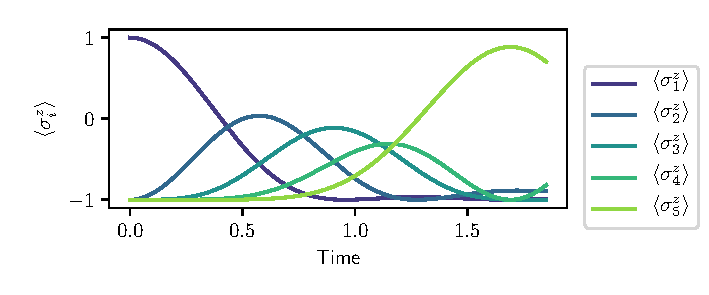
\includegraphics{alltheplots/j_const/expval_z.pdf}
    \caption{Time Evolution of the individual magnetizations of the qubits
    $\expval{\sigma^z_i}$.
    The first qubit ($i=1$) is prepared to be in the excited state at $t=0$ and all the others
    are in the ground state.}
    \label{fig:hom_magn}
\end{figure}\\
We can clearly see in \cref{fig:hom_magn} that the first qubit continuously loses while the next qubit gains magnetization.
But since the second one interacts with its next neighbor as well, it quickly gives up its magnetization.
This continues to the last qubit, where the magnetization builds up again. Thus, the state essentially propagates through
the chain.\\ Though it has to be noted that the state does not \emph{perfectly} transfer through the chain.
Let us confer with \cref{fig:hom_fide}, which shows the fidelity and the Kullback-Leibler divergence between
the state of the first qubit at time $t=0$ and the state of the last qubit as a function of time.
Recall from \cref{sec:entropy-rel-quant} that the Kullback-Leibler divergence and the fidelity of two
identical density matrices are $0$ and $1$ respectively.
Note that we use $S(\rho_1(0)\mid\mid\rho_N(t))$ instead of $S(\rho_N(t)\mid\mid\rho_1(0))$. Since our first qubit is in the excited state,
its density matrix is non-invertible. The term $\Trace[\rho_N(t)\ln(\rho_1(0))]$ of the relative entropy (cf. \cref{def:}) 
logarithmic scaling for the Kullback-Leibler divergence. We choose this, because are interested in the
relative entropy close to zero and since the qubits start out in perfectly different states, i.e. their relative entropy at the initial conditions is infinite,
the values of $S(\rho_1(0)\mid\mid\rho_N(t))$ vary by several orders of magnitude.
\begin{figure}[h!]
    \centering
    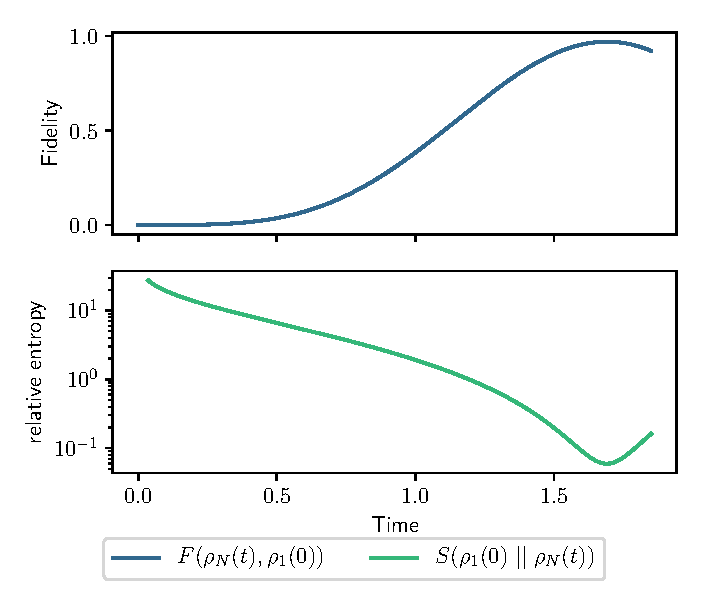
\includegraphics{alltheplots/j_const/fidelity_kld_fixed_legend.pdf}
    \caption{Time dependent Fidelity and Kullback-Leibler Divergence (relative entropy) between the first and last qubit.
    $F(\rho_N(t), \rho_1(0))$ denotes the Fidelity between the initial state of the first qubit and the time evolution of the last qubit.
    Likewise, $S(\rho_1(0)\mid\mid\rho_N(t))$ \textcolor{red}{check yourself before you wreck yourself} denotes the relative entropy between the initial state of the first qubit and the time evolution of the last qubit.}
    \label{fig:hom_fide}
\end{figure}\\
\Cref{fig:hom_fide} shows that the state does not transfer perfectly through the chain.
Additionally, we see that the flow reverses, i.e. the second to last qubit builds up magnetization again.
This is an important consideration if we want to verify Pendry's inequality, \cref{ineq:pendry-bound}.
If the dynamics of the chain reverse and the transfer begins anew, starting from the last qubit,
all the available information has to have been passed on to the last one.
Since the original derivation considered information as the detection of a particle \cite{BA_Pendry_1983}, 
our investigation concerns itself up to the point to which the transfer happened and the 
We therefore determine the time at which the dynamics reverse and verify \cref{ineq:pendry-bound} up to this time.
We define the information flow as the time derivative of the von Neumann entropy of the last qubit,
i.e. the change in average uncertainty over time.
If the information about the state of the first qubit propagates through the chain, the last qubit will 
In \cref{fig:hom_pendry} the energy flow, multiplied with $\pi/(3\ln^2(2))$, and the squared information flow are shown as a function of time.
The grey lines are drawn into the plot as visual aids. The horizontal lines denotes $0$ and the vertical line denotes the
time at which the dynamics of the chain reverses.
\begin{figure}[h!]
    \centering
    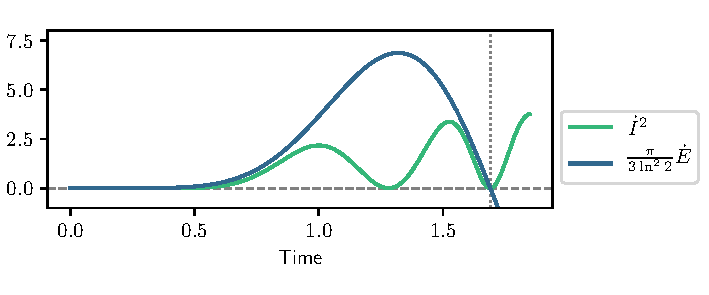
\includegraphics{alltheplots/j_const/pendry_grey_lines_fixed_legend.pdf}
    \caption{Energy flow multiplied with a constant factor and squared information flow of the last qubit. The dotted line
    indicates the time up to which Pendry's inequality \cite{BA_Pendry_1983} was verified.}
    \label{fig:hom_pendry}
\end{figure}\\
\Cref{fig:hom_pendry} clearly shows that the energy flow and information flow obey the expected behaviour from \cref{ineq:pendry-bound}.
The inequality holds up until the dynamics reverse.\\
We can also infer from \cref{fig:hom_pendry} that the inequality 
But since we prepared the first qubit of our system in the excited state, this was the largest possible information flow, if we prepare
all the other qubits in the ground state. That means that we need to tweak our system in a way such that the state gets transfered faster or better.
\section{Perfect state transfer}\label{sec:perfect-state-transfer}
Hamiltonian \cite{BA_Christandl_2004}\\
because this is the fastest state transfer \cite{Ba_QUANTUM-SPEED-LIM}
\begin{align}\label{eq:hamiltonian-perfect-transfer}
    \hat{H} = -\sum\limits_i \omega\sigma^z_i + \sum\limits_i \frac{J_i}{2} (\sigma^x_i\sigma^x_{i+1}+\sigma^y_i\sigma^y_{i+1})\qq{with}
    J_i = \frac{1}{2}\sqrt{i(N-i)}
\end{align}
\begin{figure}[h!]
    \centering
    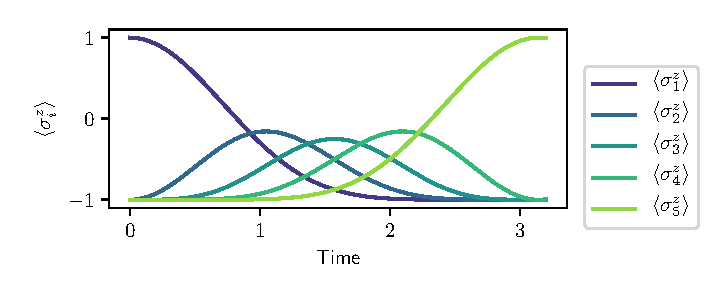
\includegraphics{alltheplots/j_var/expval_z.pdf}
    \caption{Time evolution of $\expval{\sigma^z_i}$}
    \label{fig:perf_expval_z}
\end{figure}
\begin{figure}[h!]
    \centering
    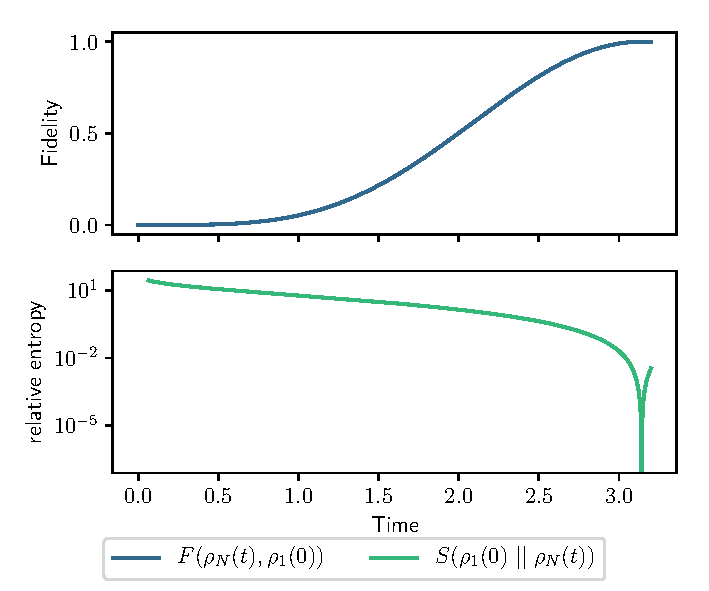
\includegraphics{alltheplots/j_var/fidelity_kld_fixed_legend.pdf}
    \caption{Time dependent Fidelity and Kullback-Leibler divergence (relative entropy) between the first and last qubit.
    $F(\rho_N(t), \rho_1(0))$ denotes the Fidelity between the initial state of the first qubit and the time evolution of the last qubit.
    Likewise, $S(\rho_1(0)\mid\mid\rho_N(t))$ denotes the relative entropy between the initial state of the first qubit and the time evolution of the last qubit.}
    \label{fig:perf_fide_kld}
\end{figure}
\begin{figure}[h!]
    \centering
    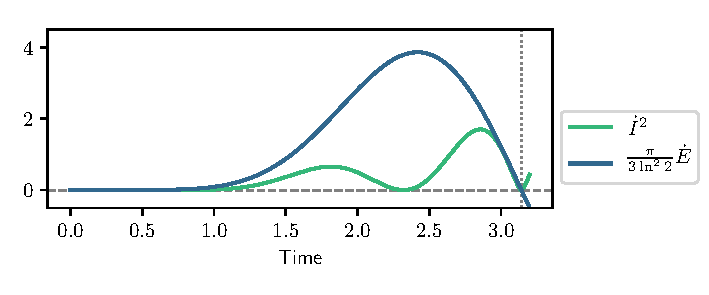
\includegraphics{alltheplots/j_var/pendry_grey_lines_fixed_legend.pdf}
    \caption{Pendry bound \textcolor{red}{redo legend, grey lines?}\cite{BA_Pendry_1983}}
    \label{fig:perf_pendry}
\end{figure}
\section{Quantumn Correlations}
Hamiltonian of the previous section showed that perfect state transfer is possible and that the dynamics reverse at $t=\pi$. Let us
verify this behaviour for two initially correlated qubits, instead of one initial qubit in the excited state.
\subsection{Bell-State}
Bell state \cite{BA_HS_nielsenchuang}
\begin{align}
    \dyad{11}, \qq{with} \ket{11} = \frac{\ket{01}-\ket{10}}{\sqrt{2}}
\end{align}
\Cref{fig:bell_expval_z}
\begin{figure}[H]
    \centering
    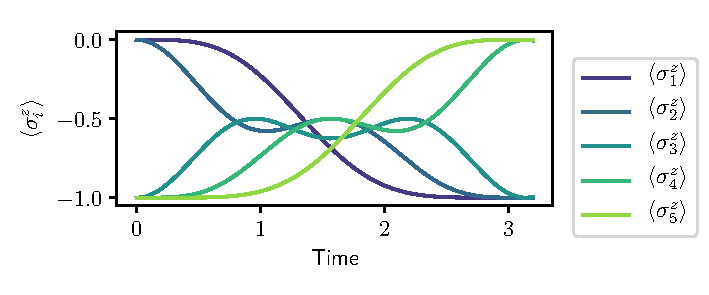
\includegraphics{alltheplots/bell/expval_z.pdf}
    \caption{Time Evolution of the individual magnetizations of the qubits
    $\expval{\sigma^z_i}$.
    The first two qubits ($i=1, i=2$) are prepared in an entangled state, namely the Bell state $\ket{\beta_{11}} = \left(\ket{01}-\ket{10}\right)/\sqrt{2}$
    at $t=0$ and all the others
    are in the ground state.}
    \label{fig:bell_expval_z}
\end{figure}
\Cref{fig:bell_fide_dkl}
\begin{figure}[H]
    \centering
    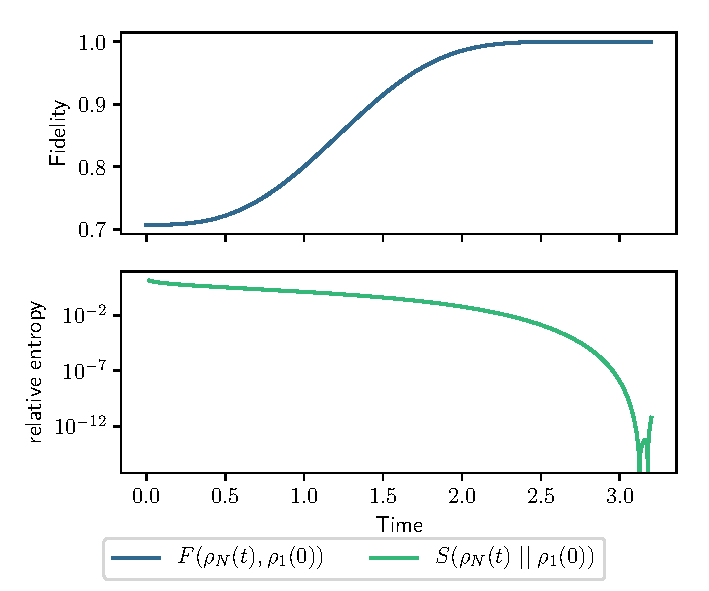
\includegraphics{alltheplots/bell/fidelity_dkl.pdf}
    \caption{Time dependent Fidelity and Kullback-Leibler divergence (relative entropy) between the first and last qubit.
    $F(\rho_N(t), \rho_1(0))$ denotes the Fidelity between the initial state of the first qubit and the time evolution of the last qubit.
    Likewise, $S(\rho_N(t)\mid\mid\rho_1(0))$ denotes the relative entropy between the initial state of the first qubit and the time evolution of the last qubit.}
    \label{fig:bell_fide_dkl}
\end{figure}
Pendrybound
\Cref{fig:bell_pendry}
\begin{figure}[H]
    \centering
    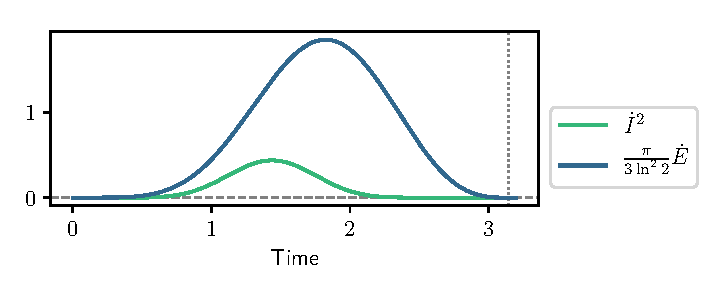
\includegraphics{alltheplots/bell/pendry_grey_lines.pdf}
    \caption{Energy flow multiplied with a constant factor and squared information flow of the last qubit. The dotted line
    indicates the time up to which Pendry's inequality \cite{BA_Pendry_1983} was verified.}
    \label{fig:bell_pendry}
\end{figure}
\textbf{TODO: THIS SECTION}
\subsection{Correlations}\label{sec:therm-corr}
correlations from \cite{BA_kaonan_correlations}:
\begin{align}\label{eq:kaonans-corr}
    \chi = -i\alpha(\sigma^+_k \sigma^-_{k+1} - \sigma^-_k \sigma^+_{k+1})
\end{align}
The correlations in \cref{eq:kaonans-corr} have been shown to be experimentally realizable \cite{BA_kaonan_correlations}.
\textcolor{red}{\textbf{CALCULATE $\vb*{\alpha}$ EXPLICITLY}}
Hamiltonian from \cref{sec:perfect-state-transfer}, because it has the nice periodic behaviour.\\
At first we consider the two qubits at the same inverse temperature $\beta$.
\begin{figure}[h!]
    \centering
    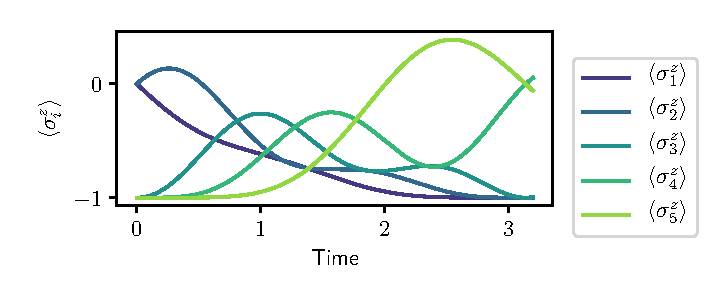
\includegraphics{alltheplots/corr_at_diff_pos-new-alpha/12_expval_z.pdf}
    \caption{Time Evolution of the individual magnetizations of the qubits
    $\expval{\sigma^z_i}$.
    The first two qubits ($i=1, i=2$) are prepared in an initially correlated state $\rho_{12} = \rho_1 \otimes \rho_2 + \chi$
    and all the others are in the ground state.}
    \label{fig:corr12_expval_z}
\end{figure}\\
1234
\begin{figure}[h!]
    \centering
    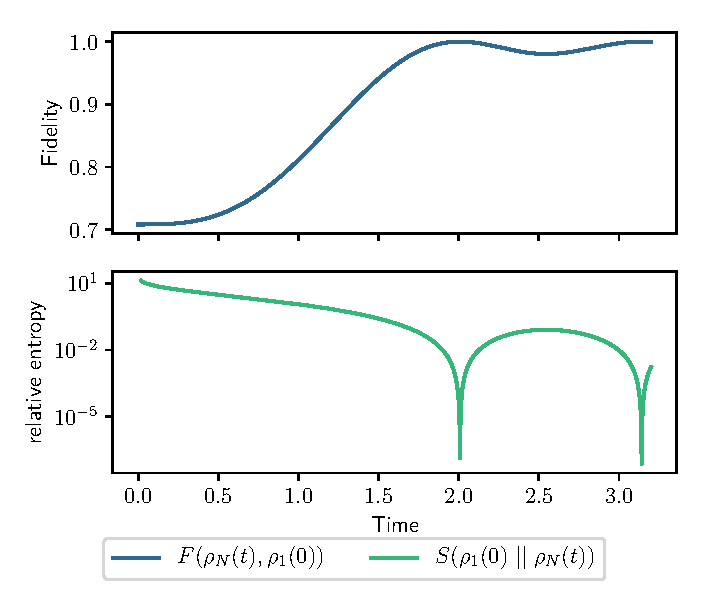
\includegraphics{alltheplots/corr_at_diff_pos-new-alpha/12_fidelity_kld.pdf}
    \caption{Fidelity and KLD}
    \label{fig:corr12_fid_kld}
\end{figure}\\
1234
\begin{figure}[h!]
    \centering
    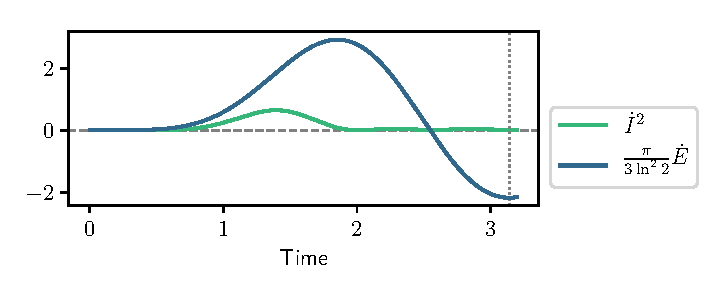
\includegraphics{alltheplots/corr_at_diff_pos-new-alpha/12_pendry_grey_lines.pdf}
    \caption{Pendry bound \cite{BA_Pendry_1983}}
    \label{fig:corr12_pendry}
\end{figure}\\

\subsection{Thermal correlations at different positions in the chain}
\textcolor{red}{\textbf{THINK OF A BETTER SUBSECTION TITLE}}\\
We have seen that the bound breaks before all the information of the first state gets passed on to the last one.
How does it look like for the correlations at a different position?
Correlations at positions 2 and 3:
\begin{figure}[h!]
    \centering
    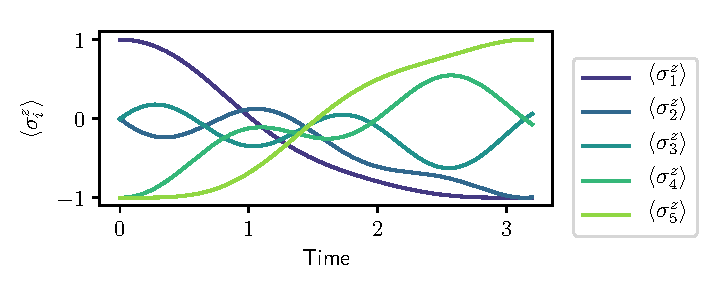
\includegraphics{alltheplots/corr_at_diff_pos-new-alpha/23_expval_z.pdf}
    \caption{Time Evolution of the individual magnetizations of the qubits
    $\expval{\sigma^z_i}$.
    The first two qubits ($i=1, i=2$) are prepared in an initially thermally correlated state $\rho_{12} = \rho_1 \otimes \rho_2 + \chi$
    and all the others are in the ground state.}
    \label{fig:corr23_expval_z}
\end{figure}\\
1234
\begin{figure}[h!]
    \centering
    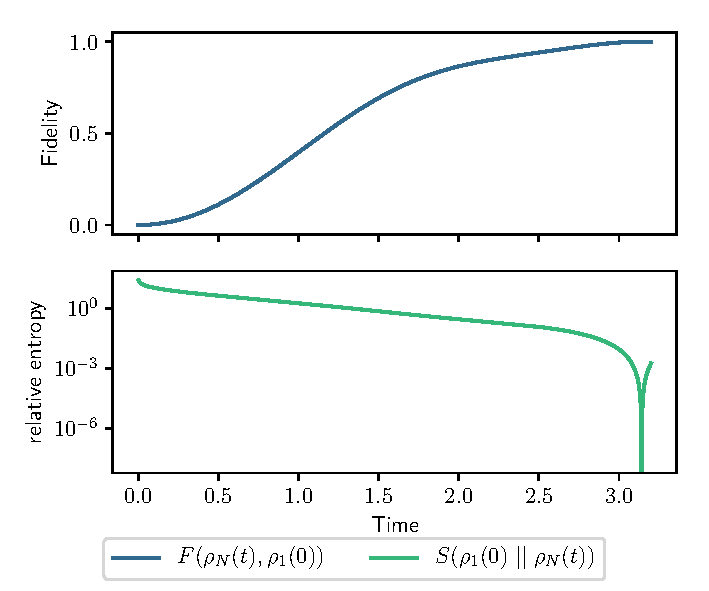
\includegraphics{alltheplots/corr_at_diff_pos-new-alpha/23_fidelity_kld.pdf}
    \caption{Fidelity and KLD}
    \label{fig:corr23_fid_kld}
\end{figure}\\
1234
\begin{figure}[h!]
    \centering
    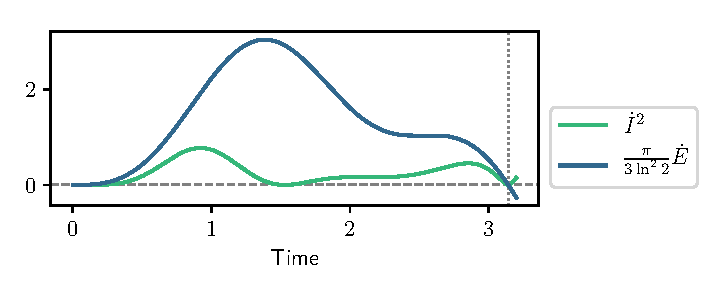
\includegraphics{alltheplots/corr_at_diff_pos-new-alpha/23_pendry_grey_lines.pdf}
    \caption{Pendry bound \cite{BA_Pendry_1983}}
    \label{fig:corr23_pendry}
\end{figure}
3 and 4:
\begin{figure}[h!]
    \centering
    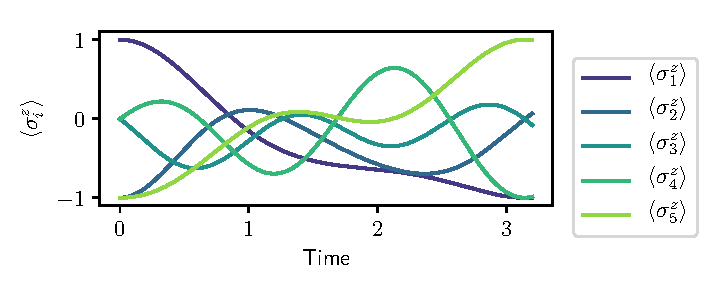
\includegraphics{alltheplots/corr_at_diff_pos-new-alpha/34_expval_z.pdf}
    \caption{Time Evolution of the individual magnetizations of the qubits
    $\expval{\sigma^z_i}$.
    The first two qubits ($i=1, i=2$) are prepared in an initially thermally correlated state $\rho_{12} = \rho_1 \otimes \rho_2 + \chi$
    and all the others are in the ground state.}
    \label{fig:corr34_expval_z}
\end{figure}\\
1234
\begin{figure}[h!]
    \centering
    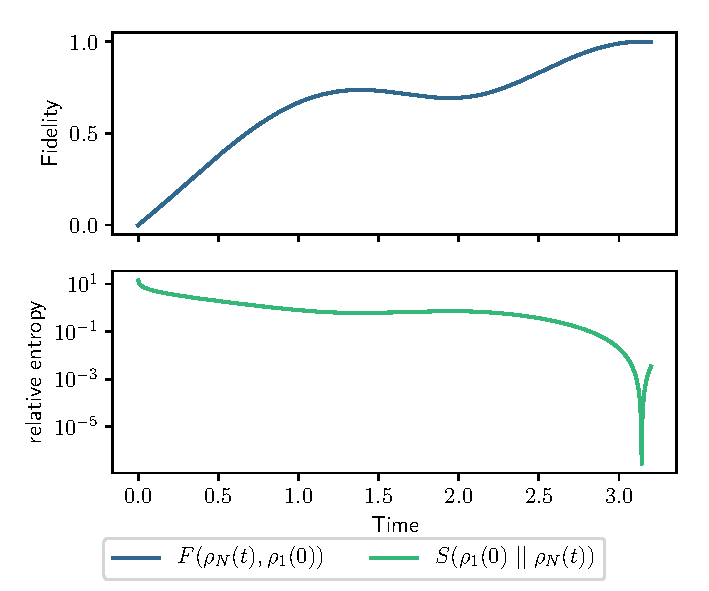
\includegraphics{alltheplots/corr_at_diff_pos-new-alpha/34_fidelity_kld.pdf}
    \caption{Fidelity and KLD}
    \label{fig:corr34_fid_kld}
\end{figure}\\
1234
\begin{figure}[h!]
    \centering
    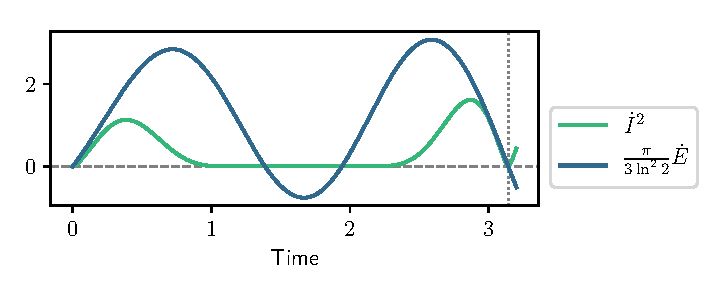
\includegraphics{alltheplots/corr_at_diff_pos-new-alpha/34_pendry_grey_lines.pdf}
    \caption{Pendry bound \cite{BA_Pendry_1983}}
    \label{fig:corr34_pendry}
\end{figure}
4 and 5:
\begin{figure}[h!]
    \centering
    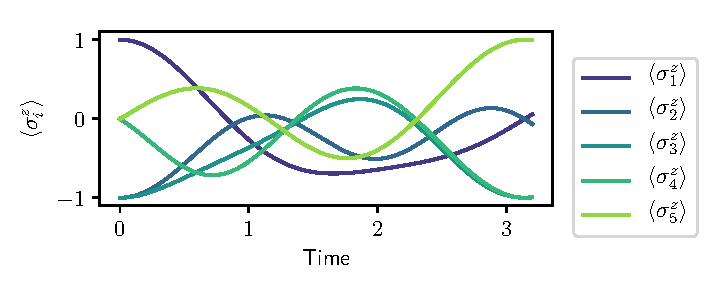
\includegraphics{alltheplots/corr_at_diff_pos-new-alpha/45_expval_z.pdf}
    \caption{Time Evolution of the individual magnetizations of the qubits
    $\expval{\sigma^z_i}$.
    The first two qubits ($i=1, i=2$) are prepared in an initially thermally correlated state $\rho_{12} = \rho_1 \otimes \rho_2 + \chi$
    and all the others are in the ground state.}
    \label{fig:corr45_expval_z}
\end{figure}\\
1234
\begin{figure}[h!]
    \centering
    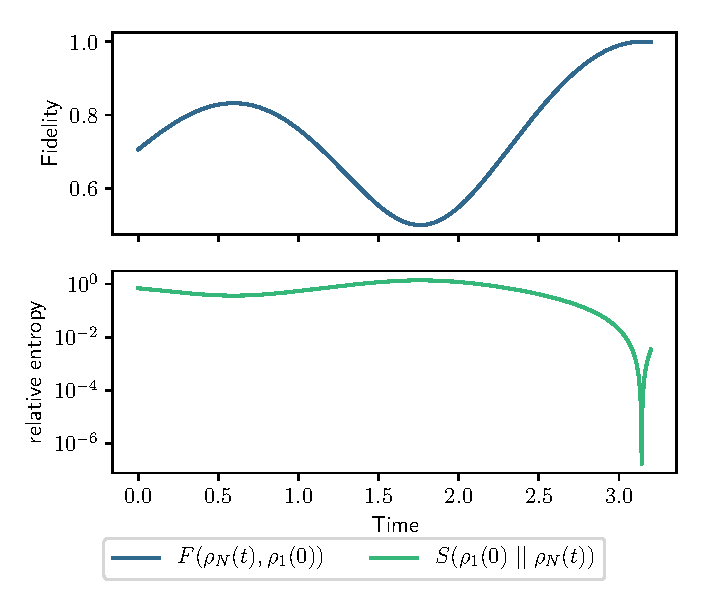
\includegraphics{alltheplots/corr_at_diff_pos-new-alpha/45_fidelity_kld.pdf}
    \caption{Fidelity and KLD}
    \label{fig:corr45_fid_kld}
\end{figure}\\
1234
\begin{figure}[h!]
    \centering
    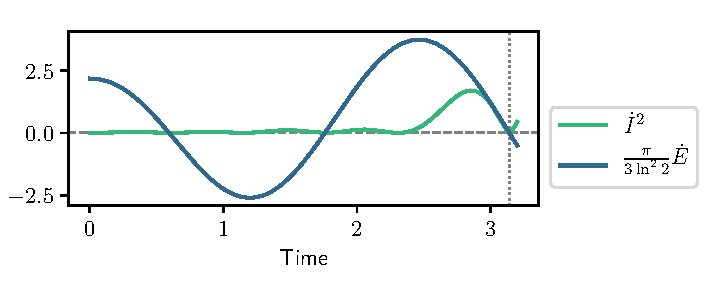
\includegraphics{alltheplots/corr_at_diff_pos-new-alpha/45_pendry_grey_lines.pdf}
    \caption{Pendry bound \cite{BA_Pendry_1983}}
    \label{fig:corr45_pendry}
\end{figure}
\subsection{Dependence of the correlations on the Temperature}\label{sec:diff-beta}
So far, we have discussed only initial correlations of states with identical thermal states, i.e. the identical inverse temperature $\beta$.
In this section we will investigate the behaviour of the chain, where the two initially correlated qubits do not have the same inverse
temperature.
First, we will consider the case where $\beta_1 < \beta_2$, i.e. the temperature of the first qubit is \emph{larger} than the second.
Note that for $\beta \gg 1$ the thermal state approaches the ground state.
\begin{figure}[h!]
    \centering
    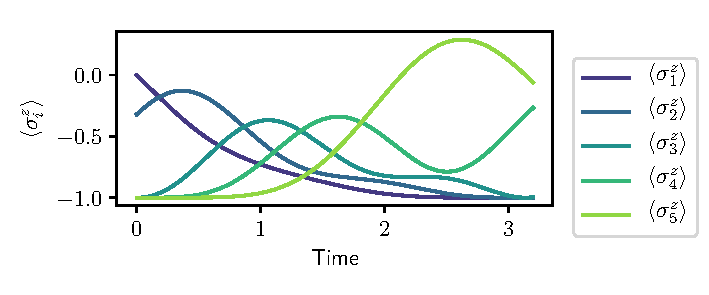
\includegraphics{alltheplots/diff_beta/beta1<beta2/12_expval_z.pdf}
    \caption{Time Evolution of the individual magnetizations of the qubits
    $\expval{\sigma^z_i}$.
    The first two qubits ($i=1, i=2$) are prepared in an initially thermally correlated state $\rho_{12} = \rho_1 \otimes \rho_2 + \chi$
    and all the others are in the ground state.}
    \label{fig:beta1_lt_beta2_corr12_expval_z}
\end{figure}\\
1234
\begin{figure}[h!]
    \centering
    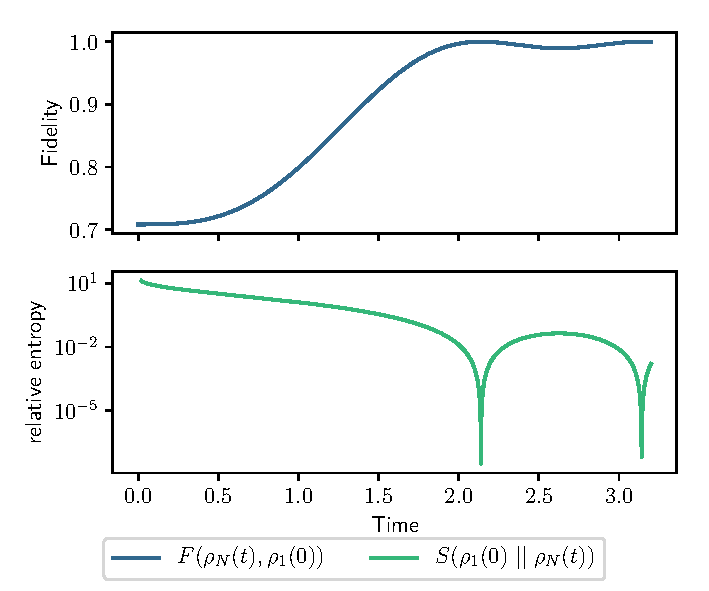
\includegraphics{alltheplots/diff_beta/beta1<beta2/12_fidelity_kld.pdf}
    \caption{Fidelity and KLD}
    \label{fig:beta1_lt_beta2_corr12_fid_kld}
\end{figure}\\
1234
\begin{figure}[h!]
    \centering
    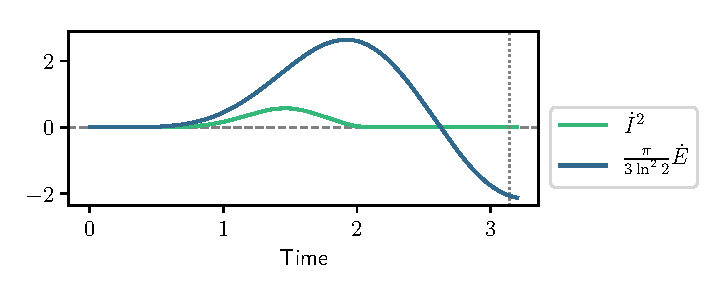
\includegraphics{alltheplots/diff_beta/beta1<beta2/12_pendry_grey_lines.pdf}
    \caption{Pendry bound \cite{BA_Pendry_1983}}
    \label{fig:beta1_lt_beta2_corr12_pendry}
\end{figure}\\
asdfasdswq
safda
\par
Here we consider $\beta_1 > \beta_2$.
\begin{figure}[h!]
    \centering
    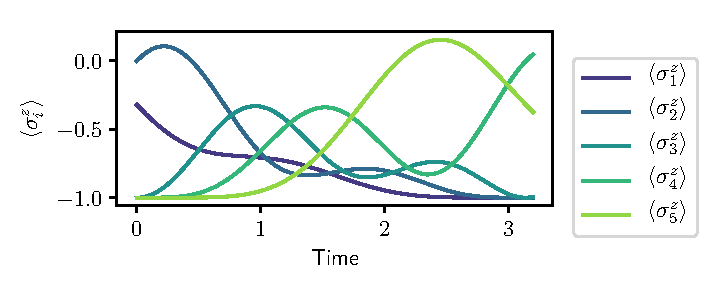
\includegraphics{alltheplots/diff_beta/beta1>beta2/12_expval_z.pdf}
    \caption{Time Evolution of the individual magnetizations of the qubits
    $\expval{\sigma^z_i}$.
    The first two qubits ($i=1, i=2$) are prepared in an initially thermally correlated state $\rho_{12} = \rho_1 \otimes \rho_2 + \chi$
    and all the others are in the ground state.}
    \label{fig:beta1_gt_beta2_corr12_expval_z}
\end{figure}\\
1234
\begin{figure}[h!]
    \centering
    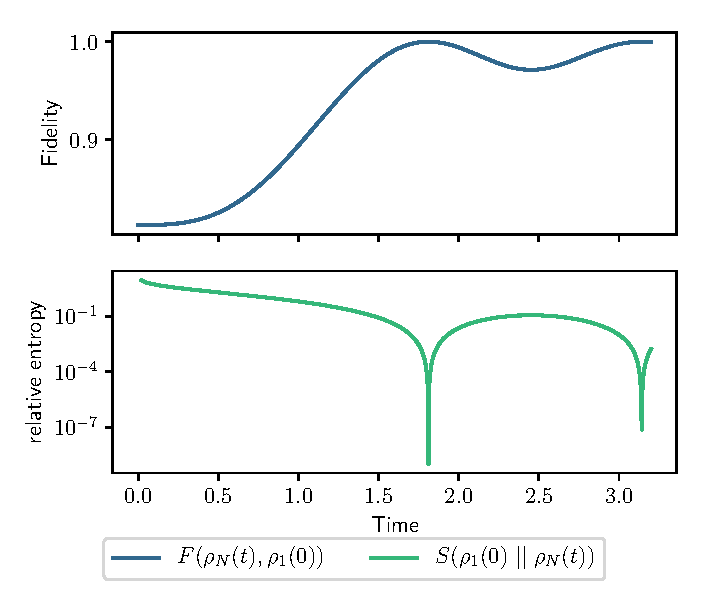
\includegraphics{alltheplots/diff_beta/beta1>beta2/12_fidelity_kld.pdf}
    \caption{Fidelity and KLD}
    \label{fig:beta1_gt_beta2_corr12_fid_kld}
\end{figure}\\
1234
\begin{figure}[h!]
    \centering
    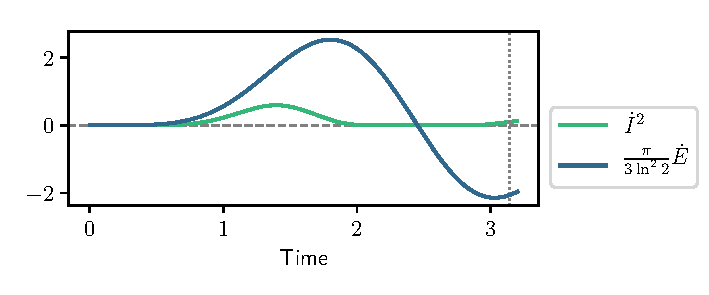
\includegraphics{alltheplots/diff_beta/beta1>beta2/12_pendry_grey_lines.pdf}
    \caption{Pendry bound \cite{BA_Pendry_1983}}
    \label{fig:beta1_gt_beta2_corr12_pendry}
\end{figure}\\
1234
\section{Different Maxima}
\textcolor{red}{\textbf{DEFINITELY LOOK FOR A BETTER SECTION TITLE}}
$\displaystyle\min_{t\in[0,\pi]}{\frac{\pi}{3\ln^22}\dot{E}-\dot{I}^2}$
We know that $\abs{\alpha_\text{max}}$ is bounded because of the positivity of $\rho$. What is the maximum $\alpha$ for different $\beta_{1,2}$?
\begin{figure}[h!]
    \centering
    \includegraphics{alltheplots/alpha/alphamax_3d_with_grey_lines.pdf}
    \caption{surface plot of $\alpha_\text{max}(\beta_1, \beta_2)$.}
\end{figure}

\newpage
\section{Bound on information flow with correlations}% for systems with quantum correlations}
As seen in section \cref{sec:therm-corr}, we are able to break the bound by introducing quantum correlations to our system.
It is now of interest to find a bound for $\dot{I}^2$.
In the following, subscript $\chi$ will denote observables with contributions from correlations
whereas subscript $0$ denotes observables without contributions from correlations.
Thus, the energy flow in the system with non-zero $\chi$ can be represented as
\begin{align}
    \dot{E} = \dot{E}_0^t + \dot{E}_\chi^t.
\end{align}

\begin{align}
    \dot{S} &= \beta \dot{E}^t - \dot{S}_\chi(\rho^t_N \mid \mid \rho^0_N)\label{eq:dotVN_with_chi}\\
    \dot{S}_0 &= \beta \dot{E}_0^t- \dot{S}_0(\rho^t_N \mid \mid \rho^0_N)\label{eq:dotVN_no_chi}
\end{align}
Subtracting \cref{eq:dotVN_no_chi} from \cref{eq:dotVN_with_chi} gives us
\begin{align}
    \dot{S} - \dot{S}_0 &= \beta \dot{E}^t - \dot{S}_\chi(\rho^t_N \mid \mid \rho^0_N) - \beta \dot{E}_0^t - \dot{S}(\rho^t_N \mid \mid \rho^0_N)\nonumber\\
    &= \beta \left(\dot{E}_0^t + \dot{E}_\chi^t\right) - \dot{S}_\chi(\rho^t_N \mid \mid \rho^0_N) - \beta \dot{E}_0^t + \dot{S}(\rho^t_N \mid \mid \rho^0_N)\nonumber\\
    &= \beta \dot{E}_\chi^t - \Delta_\chi \dot{S}(\rho^t_N \mid \mid \rho^0_N),
\end{align}
with
\begin{align*}
    \Delta_\chi\dot{S}(\rho^t_N \mid \mid \rho^0_N) = \dot{S}_\chi(\rho^t_N \mid \mid \rho^0_N) - \dot{S}(\rho^t_N \mid \mid \rho^0_N).
\end{align*}
\dots
Finally we get
\begin{align}\label{eq:newbound}
    \dot{S}^2 \leq \frac{\pi}{3\ln^22} \dot{E} + \beta^2 \dot{E}^t_\chi + \left(\Delta_\chi\dot{S}(\rho^t_N \mid \mid \rho^0_N)\right)^2 + 2\dot{S}_0 \dot{E}_\chi
    - 2\beta\dot{E}_\chi \Delta_\chi\dot{S}(\rho^t_N \mid \mid \rho^0_N) -2\dot{S}_0 \Delta_\chi\dot{S}(\rho^t_N \mid \mid \rho^0_N)
\end{align}
\textcolor{red}{\textbf{TODO: THIS CALCULATION}}

How does this bound look like?
\begin{figure}[h!]
    \centering
    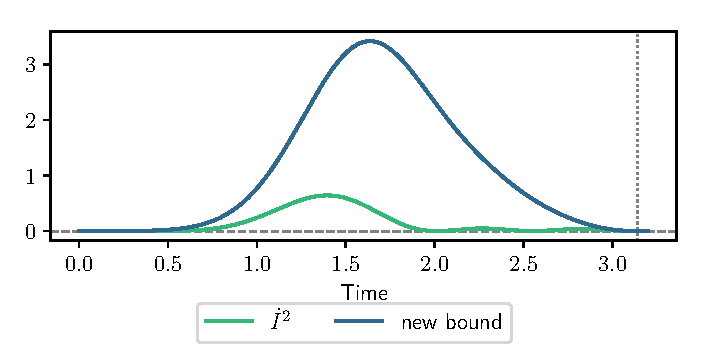
\includegraphics{alltheplots/newbound/corr12_same_beta_bound.pdf}
    \caption{new bound according to \cref{eq:newbound}}
    \label{fig:newbound_corr12_same_beta_no_old}
\end{figure}\\
Compare with old bound:
\begin{figure}[h!]
    \centering
    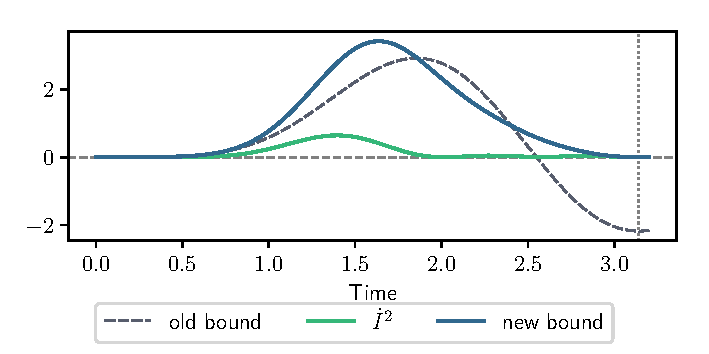
\includegraphics{alltheplots/newbound/corr12_same_beta_bound_with_old_bound.pdf}
    \caption{new bound according to \cref{eq:newbound} with old bound}
    \label{fig:newbound_corr12_same_beta_with_old} 
\end{figure}
(1,2) corr with $\beta_1<\beta_2$:
\begin{figure}[h!]
    \centering
    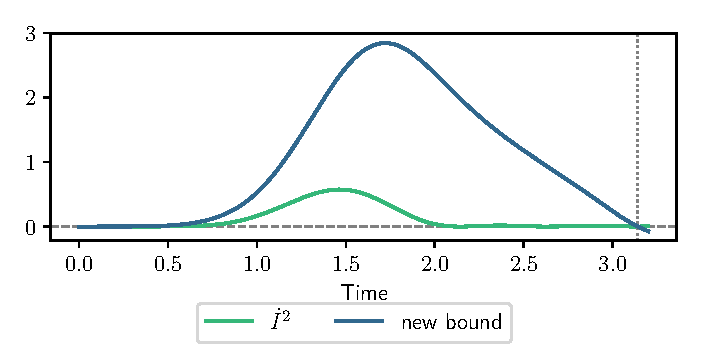
\includegraphics{alltheplots/newbound/corr12_beta1<beta2_bound_no_old_bound.pdf}
    \caption{new bound according to \cref{eq:newbound}}
    \label{fig:newbound_corr12_beta1<beta2_no_old}
\end{figure}\\
compared with old bound:
\begin{figure}[h!]
    \centering
    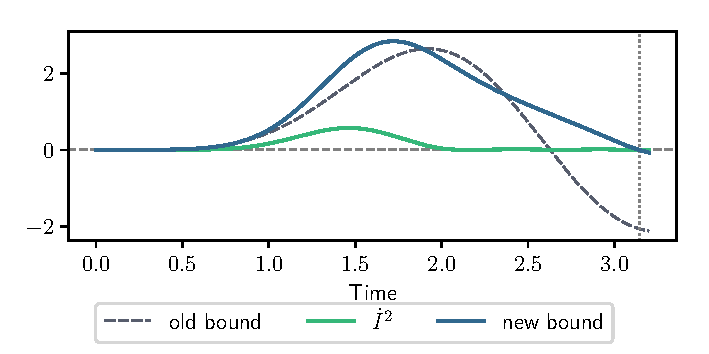
\includegraphics{alltheplots/newbound/corr12_beta1<beta2_bound_with_old_bound.pdf}
    \caption{new bound according to \cref{eq:newbound} with old bound}
    \label{fig:newbound_corr12_beta1<beta2_with_old}
\end{figure}

\section{Long range interactions}
$\partial_\alpha \dot{I}^2_\text{max}(0) \cdot \alpha/\alpha_\text{max} + \dot{I}^2_\text{max}(0)$
Long range.\cite{BA_Maier_longrange}
\begin{align}\label{eq:hamiltonian-long-range-int}
    \hat{H} = -\sum\limits_i \omega\sigma^z_i + \sum\limits_{i<j} J_ij (\sigma^+_i\sigma^-_j+\sigma^+_j\sigma^-_{i})\qq{with}
    J_{ij} = \abs{i-j}^{\alpha}\qq{and} \alpha>1
\end{align}
Magnetizations:
\begin{figure}[h!]
    \centering
    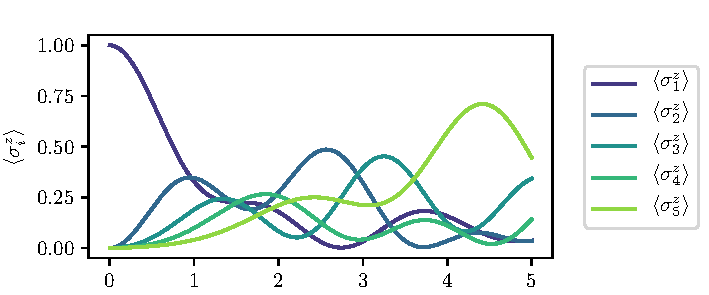
\includegraphics{alltheplots/longrange/expval_z.pdf}
    \caption{Magnetizations for long range interaction}
    \label{fig:long-expval-z}
\end{figure}
Fidelity and Kullback-Leibler
\begin{figure}[h!]
    \centering
    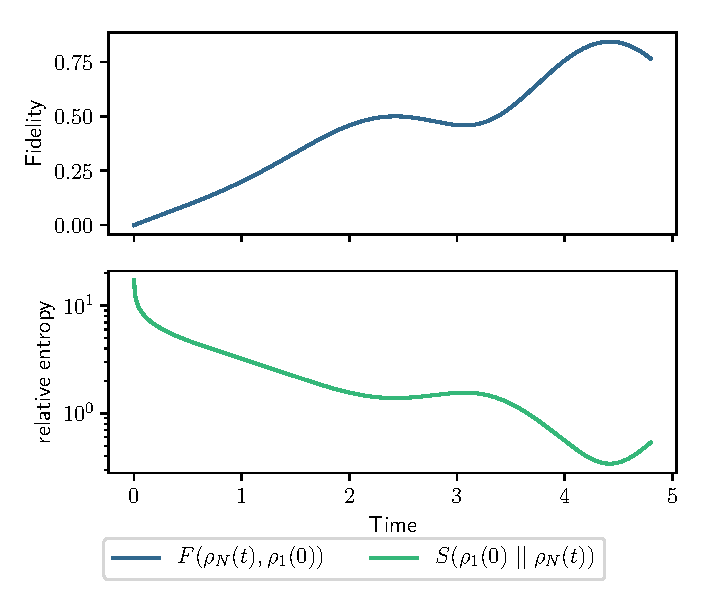
\includegraphics{alltheplots/longrange/3_fidelity_kld.pdf}
    \caption{Fidelity and Kullback-Leibler divergence}
    \label{fig:long-fid-kld}
\end{figure}
Pendrybound:
\begin{figure}[h!]
    \centering
    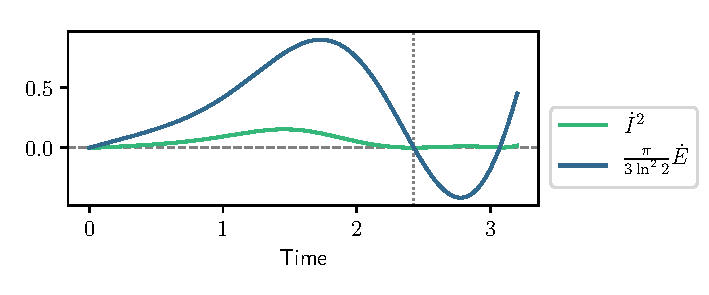
\includegraphics{alltheplots/longrange/2_pendry_grey_lines.pdf}
    \caption{Pendry bound for longrange interaction}
    \label{fig:long-pendry}
\end{figure}

\printbibliography

\declaration

\end{document}